\chapter{Pantallazos de la aplicación de ejemplo para Thin2}
\label{apendiceB}
\lhead{Apéndice B. \emph{Pantallazos de la aplicación de ejemplo para Thin2}}

\begin{figure}[h!]
\centering
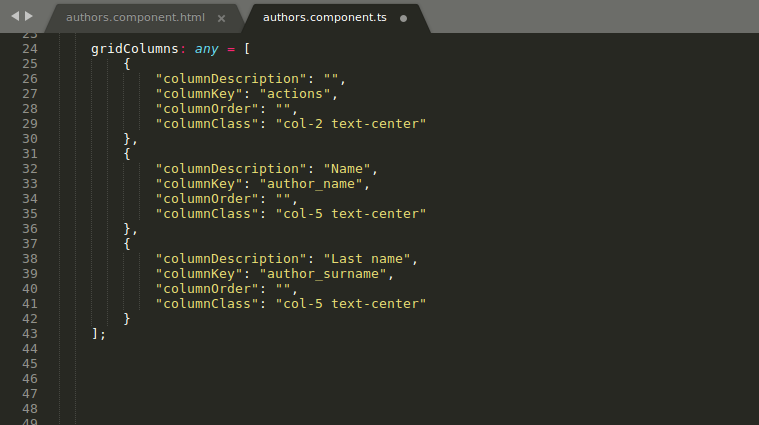
\includegraphics[width=\textwidth]{author-config}
\caption[Configuración de tabla sencilla]{Configuración de una tabla sin función.}
\label{author:1}
\end{figure}

\begin{figure}[h!]
\centering
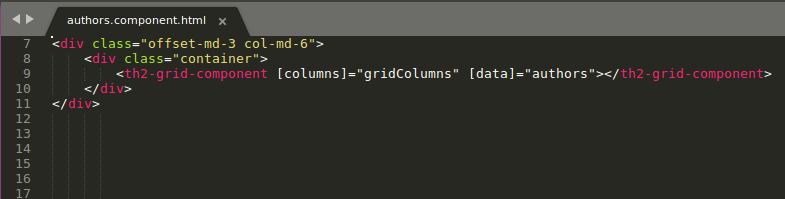
\includegraphics[width=\textwidth]{author-html}
\caption[Código html de tabla sencilla]{Código html utilizado para crear una tabla sin función.}
\label{author:2}
\end{figure}

\begin{figure}[h!]
\centering
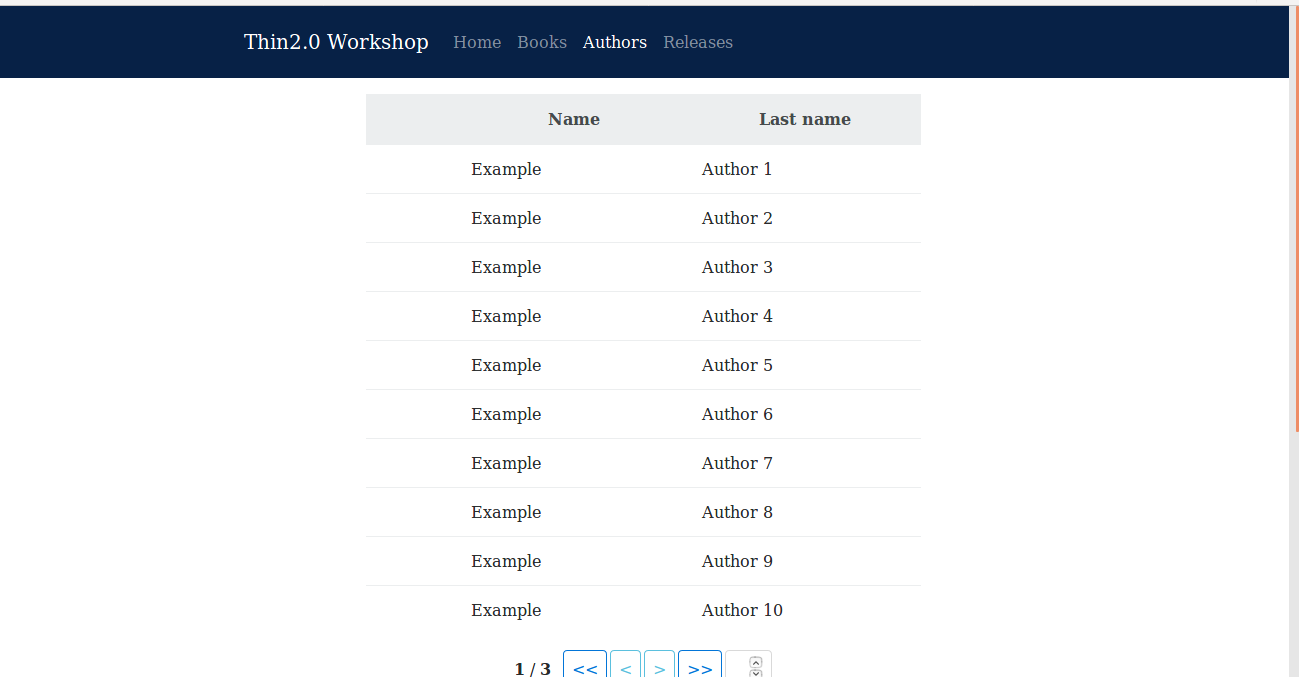
\includegraphics[width=\textwidth]{author-resultados}
\caption[Tabla sencilla en aplicación]{Resultado de la tabla realizada en la aplicación.}
\label{author:3}
\end{figure}

\begin{figure}[h!]
\centering
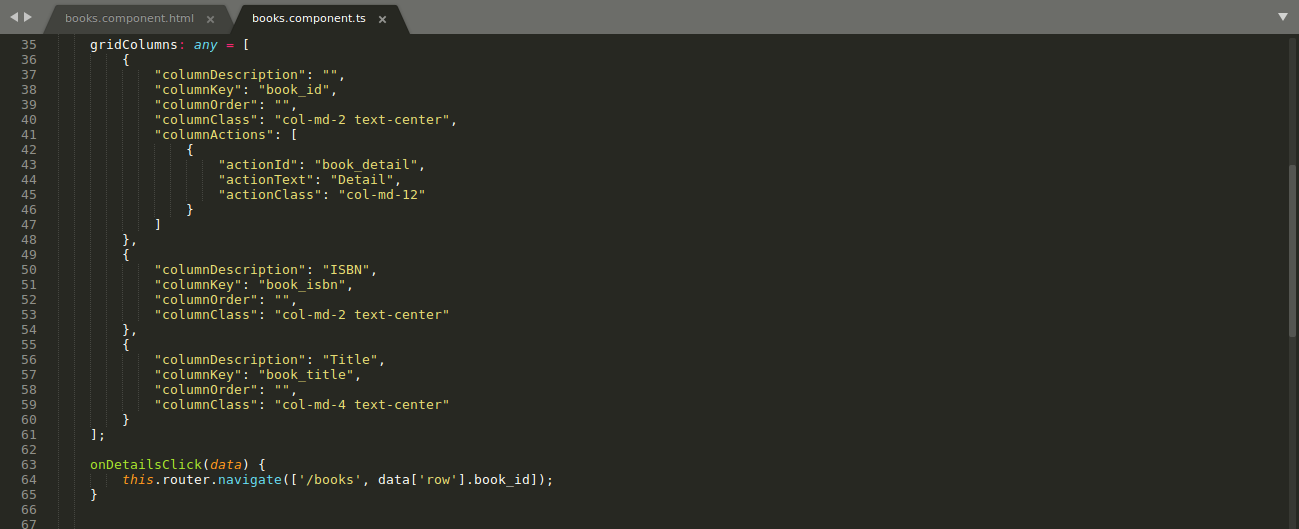
\includegraphics[width=\textwidth]{books-config}
\caption[Configuración de tabla con evento]{Configuración de una tabla con una función asociada.}
\label{books:1}
\end{figure}

\begin{figure}[h!]
\centering
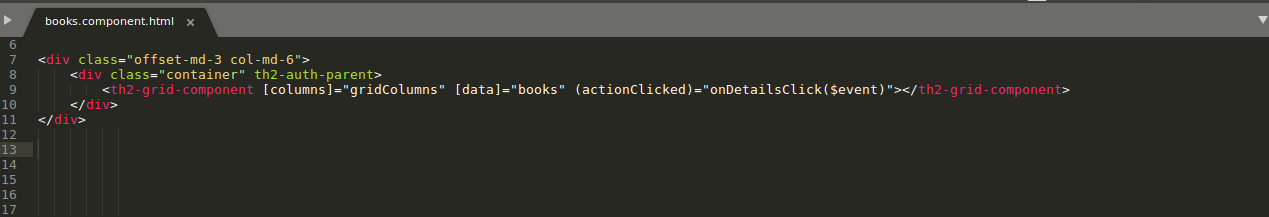
\includegraphics[width=\textwidth]{books-html}
\caption[Código html de tabla con evento]{Código html utilizado para crear una tabla con una función asociada.}
\label{books:2}
\end{figure}

\begin{figure}[h!]
\centering
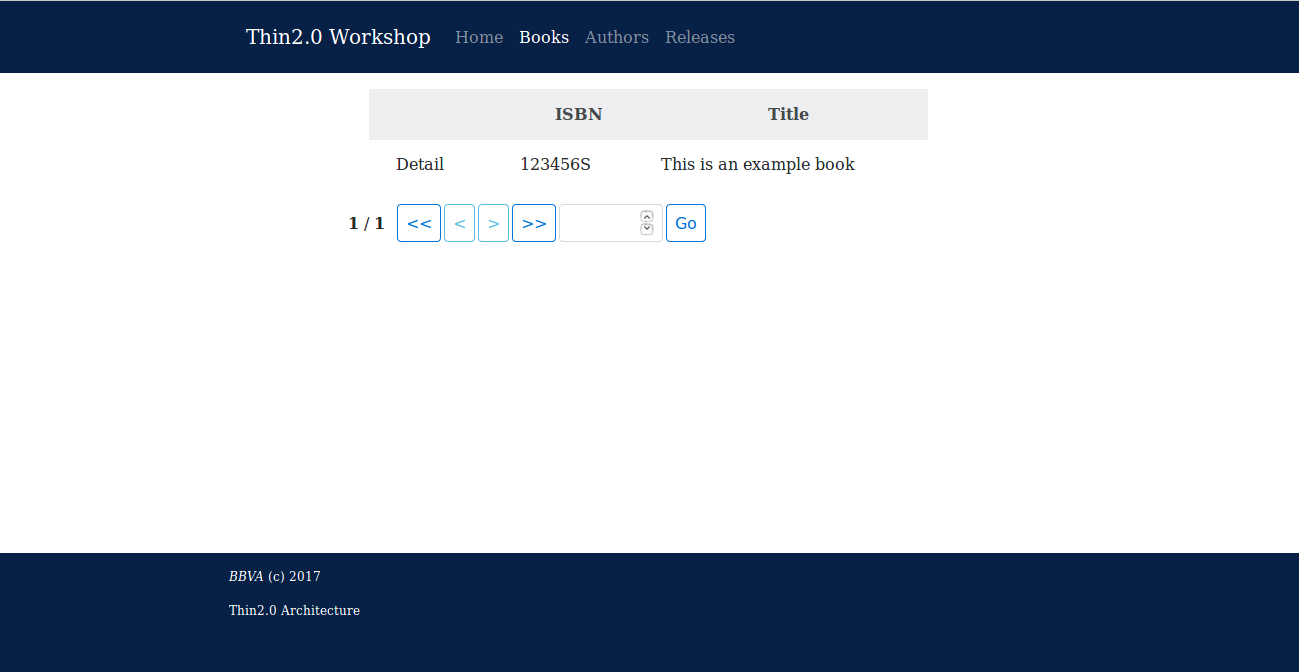
\includegraphics[width=\textwidth]{books-result}
\caption[Tabla con evento en aplicación]{Tabla con función asociada resultante en la aplicación.}
\label{books:3}
\end{figure}

\begin{figure}[h!]
\centering
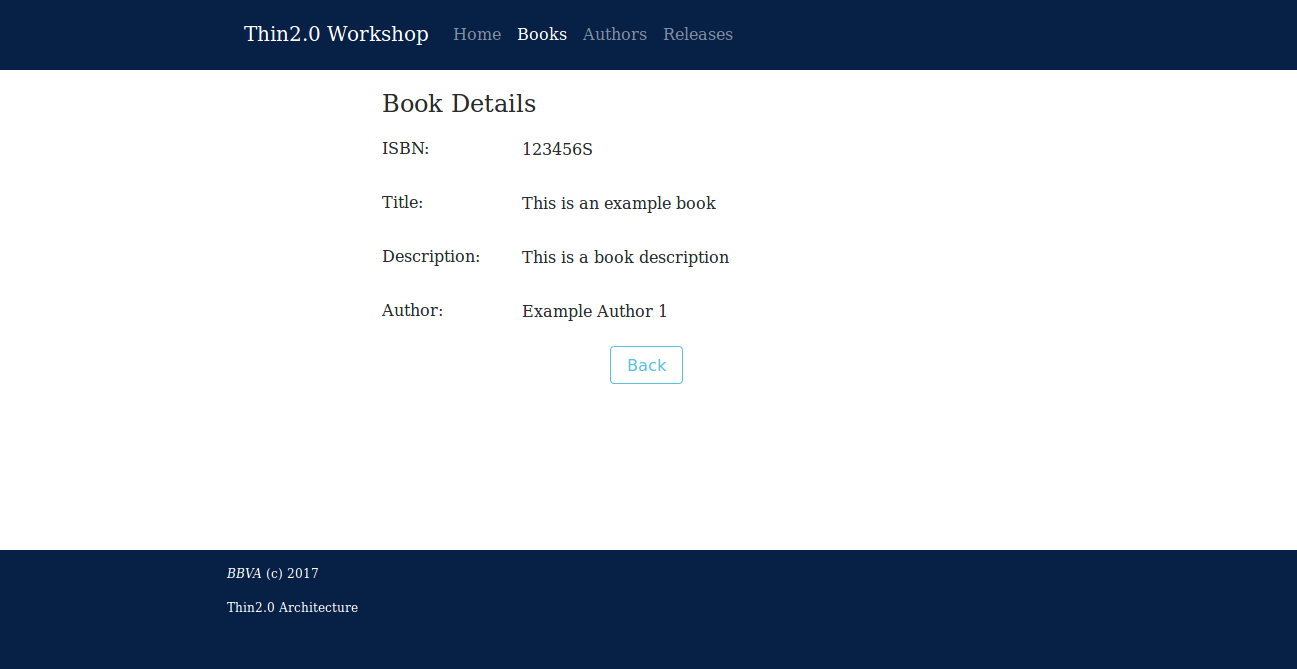
\includegraphics[width=\textwidth]{book-detail}
\caption[Página al hacer click en la tabla]{Cambio en la aplicación al ejecutar la función asociada a la celda.}
\label{books:4}
\end{figure}
